% "{'classe':('PSI'),'chapitre':'stat_pfs_3d','type':('application'),'titre':'Pied stabilisateur', 'source':'Equipe PT La Martin','comp':('B2-14','C1-05','C2-07'),'corrige':True}"
%\setchapterimage{fig_00.jpg}
\chapter*{Application \arabic{cptApplication} \\ 
Pied stabilisateur -- \ifprof Corrigé \else Sujet \fi}
\addcontentsline{toc}{section}{Application \arabic{cptApplication} : Pied stabilisateur-- \ifprof Corrigé \else Sujet \fi}

\iflivret \stepcounter{cptApplication} \else
\ifprof  \stepcounter{cptApplication} \else \fi
\fi

\setcounter{question}{0}
\marginnote{Equipe La Martinière Monplaisir.}
\begin{marginfigure}
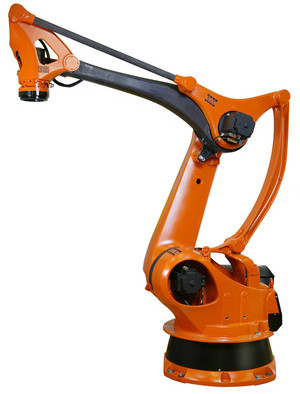
\includegraphics[width=\linewidth]{fig_01}
\end{marginfigure}

%\subsection*{Pied stabilisateur}
\ifprof
\else
On s’intéresse à un pied stabilisateur d’un engin de chantier.
La figure 1 représente l’un des 4 pieds stabilisateurs d’un engin de chantier. Chaque pied est composé d’un patin (5), de deux barres (3) et (4) et d’un vérin hydraulique (1+2) (1=corps, 2=piston). Les barres sont articulées en A et B sur le bâti (0) de l’engin et en D sur le patin. La liaison entre (1) et (2) est modélisée par une liaison pivot glissant. Toutes les autres liaisons sont considérées comme des liaisons rotules. (La pièce (5) est en liaison rotule de centre D avec les pièces (2), (3) et (4).)

\begin{center}
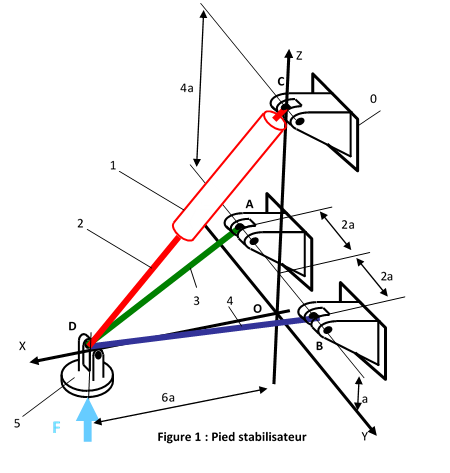
\includegraphics[width=.6\linewidth]{fig_02}\hfill
\end{center}

Extrait du diagramme des exigences :
\begin{center}
\begin{tabular}{llll}
\hline
Exigences & Critères & Niveau & Limite \\
\hline
Adaptation au vérin hydraulique	& Effort transmissible par le vérin  & \SI{60}{kN} & Maxi \\
Dimensionnement RdM & Action dans les barres & \SI{25}{kN} & Maxi \\
\hline
\end{tabular}
\end{center}

On donne $\vectf{\text{ext}}{5} = F\vect{z}$ avec $F = \SI{30000}{N}$.

La dimension $a=\SI{400}{mm}$, les points $A$, $B$ et $C$ sont dans le plan $\left(O,\vect{y},\vect{z}\right)$.
On a : $\vect{OD} = 6a\vect{x}$, $\vect{OC} = 5a\vect{z}$, $\vect{OB} = 2a\vect{y}+a\vect{z}$, $\vect{OA} = - 2a\vect{y}+a\vect{z}$. 

On pourra noter : $\vect{CD} = L_{12}\vect{x_{12}}$, $\vect{AD} = L_3\vect{x_3}$, $\vect{BD} = L_4\vect{x_4}$.
\fi

\question{Analyser le mécanisme (calculer le degré d'hyperstisme) et proposer les étapes de résolution du problème de détermination des efforts dans les liaisons.}
\ifprof
\begin{corrige}
Les pièces \{1+2\}, 3 et 4 sont bi-rotulées. Donc il existe une mobilité de rotation propre (respectivement autour de $\vect{x_{12}}$, $\vx{3}$, $\vx{4}$.
La pièce 5 peut faire 3 mouvements de rotation.

Au final, $m=6$.

Il y a 6 liaisons rotules; donc 18 inconnues statiques. 

Il y a 4 pièces que l'on peut isoler, donc 24 équations statiques. 

Au final, $h = m-E_S+I_S = 6 -24 + 18 = 0$. Le système est isostatique. On peut calculer toutes les actions mécaniques.

\vspace{.5cm}

Le torseur d'une liaison rotule, en statique est un glisseur. 

Les ensembles \{1+2\}, 3 et 4 sont tous 3 soumis à deux glisseurs. 

En appliquant le PFS à chacun de ces ensembles, on a : 
$\torseurstat{T}{2}{5} = \torseurl{F_2\vect{x_{12}}}{\vect{0}}{D}$,
$\torseurstat{T}{3}{5} = \torseurl{F_3\vect{x_3}}{\vect{0}}{D}$,
$\torseurstat{T}{4}{5} = \torseurl{F_4\vect{x_4}}{\vect{0}}{D}$.

On isole alors 5 soumis à 4 actions mécaniques. 
On applique le TRS en projection sur $\vx{0}$, $\vy{0}$, $\vz{0}$. 
\end{corrige}
\else
\fi


\question{Calculer les actions exercées par le patin sur les barres et le vérin.}
\ifprof
\begin{corrige}
On a $\vect{x_{12}} = \dfrac{\vect{CD}}{||\vect{CD}||}$
$ =\dfrac{1}{\sqrt{36a^2+25a^2}} \begin{pmatrix}6a \\ 0 \\ -5a \end{pmatrix}$ 
$= \dfrac{1}{\sqrt{61}} \begin{pmatrix}6 \\ 0 \\ -5 \end{pmatrix}$.


On a $\vect{x_{3}} = \dfrac{\vect{AD}}{||\vect{AD}||}$
$ =\dfrac{1}{\sqrt{4a^2+a^2 +36a^2}} \begin{pmatrix}6a \\ 2a \\ -a \end{pmatrix}$ 
$= \dfrac{1}{\sqrt{41}} \begin{pmatrix}6 \\ 2 \\ -1 \end{pmatrix}$.

On a $\vect{x_{4}} = \dfrac{\vect{BD}}{||\vect{BD}||}$
$ =\dfrac{1}{\sqrt{36a^2+4a^2 +a^2}} \begin{pmatrix}6a \\ -2a \\ -a \end{pmatrix}$ 
$= \dfrac{1}{\sqrt{41}} \begin{pmatrix}6 \\ -2 \\ -1 \end{pmatrix}$.

En isolant 5 et en appliquant le TRS, on a donc :
$
\left\{
\begin{array}{l}
\dfrac{6F_2}{\sqrt{61}}	+\dfrac{6F_3}{\sqrt{41}}	+\dfrac{6F_4}{\sqrt{41}}=0 \\
0		+\dfrac{2F_3}{\sqrt{41}}	-\dfrac{2F_4}{\sqrt{41}}=0 \\
-\dfrac{5F_2}{\sqrt{61}}	-\dfrac{F_3}{\sqrt{41}}		-\dfrac{F_4}{\sqrt{41}} + F=0 \\
\end{array}
\right.
$

D'après la résultante sur $\vect{y}$, $F_3=F_4$; donc 
$
\left\{
\begin{array}{l}
\dfrac{6F_2}{\sqrt{61}}	+\dfrac{12F_3}{\sqrt{41}} =0 \\
-\dfrac{5F_2}{\sqrt{61}}	-\dfrac{2F_3}{\sqrt{41}} + F=0 \\
\end{array}
\right.
$

Par suite, 
$
\left\{
\begin{array}{l}
\dfrac{6F_2}{\sqrt{61}}	+\dfrac{12F_3}{\sqrt{41}} =0 \\
-\dfrac{30F_2}{\sqrt{61}}	-\dfrac{12F_3}{\sqrt{41}} + 6F=0 \\
\end{array}
\right.
$; donc $-\dfrac{24F_2}{\sqrt{61}} + 6F=0 $ et 
${F_2} = F \dfrac{\sqrt{61}}{4}$.

Enfin, 
$F_3 = -\dfrac{F_2\sqrt{41}}{2\sqrt{61}}$ 
$= -F \dfrac{\sqrt{61}}{4} \dfrac{\sqrt{41}}{2\sqrt{61}}$
$= -F  \dfrac{\sqrt{41}}{8}$
\end{corrige}
\else
\fi


\question{Réaliser l’application numérique.}
\ifprof
\begin{corrige}
$F_2 = \SI{58576}{N}$, $F_3 = F_4 = -\SI{24011}{N}$, 
\end{corrige}
\else
\fi

\question{Les exigences du cahier des charges sont-elles vérifiées ?}
\ifprof
\begin{corrige}
Dans les barres 3 et 4 l'action maximale n'est pas dépassée. 
De plus, le vérin hydraulique est adapté à l'effort.
Les deux exigences sont donc vérifiées. 

\end{corrige}
\else
\fi

\ifcolle
\else
Eléments de correction :
\begin{enumerate}
\item $h=0$.
\item $F_2 = F \dfrac{\sqrt{61}}{4}$, $F_3 = F_4 = -F  \dfrac{\sqrt{41}}{8}$.
\item .
\item .
\end{enumerate}
\fi